\documentclass[10pt]{beamer}
\usepackage{ragged2e} % \justifying
\usepackage{bm}
\usepackage{tensor}
\newcommand\norm[1]{\left\lVert#1\right\rVert}
\usetheme{metropolis}           % Use metropolis theme
\title{FP2: Torso Pose Estimation on the \\HRP4 Humanoid Robot}
\subtitle{Michele Cipriano, Godwin K. Peprah, Lorenzo Vianello}
\date{}
\author{\textit{Supervisor:} Nicola Scianca\\
    \textit{Professors:} Giuseppe Oriolo, Alessandro De Luca\\}
\institute{Autonomous and Mobile Robotics, Robotics 2\\
    Department of Computer, Control and Management
    Engineering\\Sapienza University of Rome}

% Fontsize of figure smaller than normalsize:
\setbeamerfont{caption}{size=\scriptsize}

\begin{document}
\nocite{*}

    \maketitle

    \begin{frame}{Introduction}
        Intro.
    \end{frame}

    \begin{frame}{Kinematic Model}
        Todo.
    \end{frame}

    \begin{frame}{Extended Kalman Filter}
        Todo.
    \end{frame}

    \begin{frame}{Accelerometer Integration}
        Todo.
    \end{frame}

    \begin{frame}{Gyroscope Integration}
        Todo.
    \end{frame}

    \begin{frame}{IMU}
        Experiments (5.1).
    \end{frame}

    \begin{frame}[fragile]{Filtering Linear Velocities}
      Add to the state an approximated estimation of the velocity in such a way to fix drift accumulation.

      Velocity is obtained using position of the robot in 2 successive frames

        \begin{equation*}
        \bm{\dot{p}}_{t,k} \approx \bm{\dot{\hat{p}}}_{t,k} \approx \bm{\dot{\hat{p}}}_{t,k-1}
        = \frac{\bm{\hat{p}}_{t,k} - \bm{\hat{p}}_{t,k-1}}{T}
        \end{equation*}

    \end{frame}

    \begin{frame}[fragile]{Filtering Linear Velocities}

    \begin{figure}
    \caption{Improves the estimate of $(x, y)^{T}$ coordinates decreasing the error on $z$.}
    \centering
    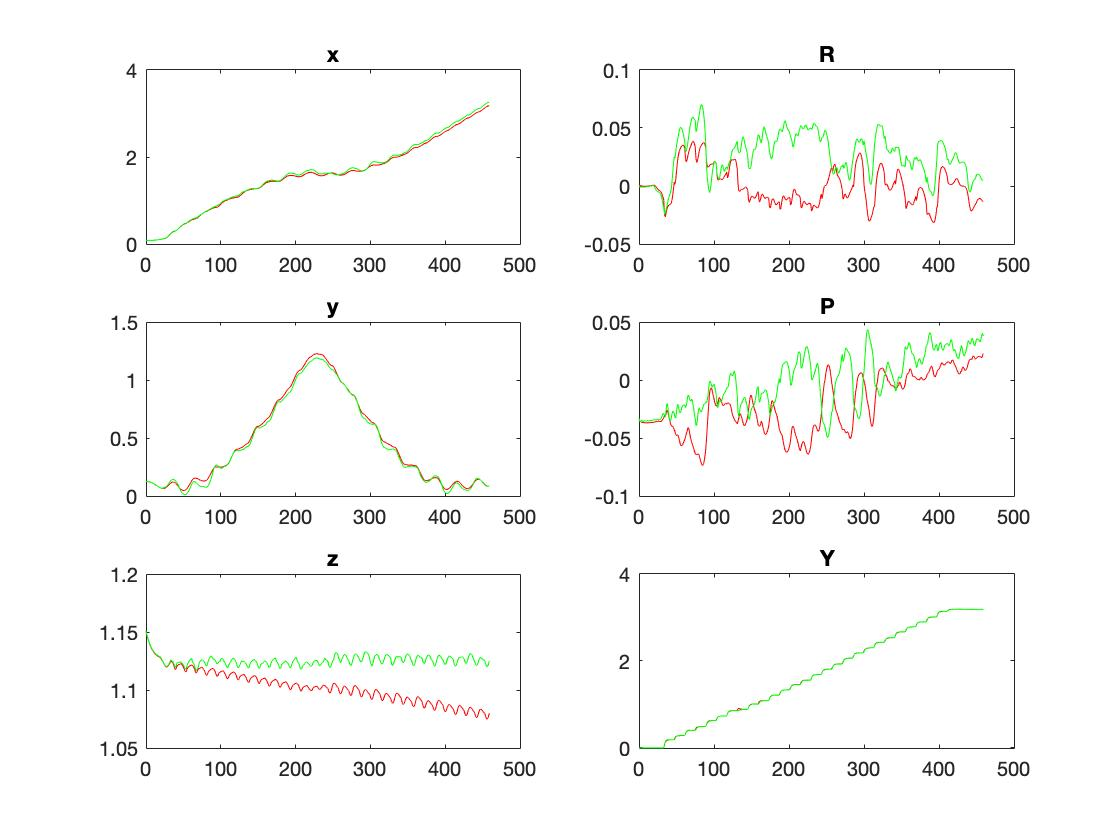
\includegraphics[width=0.5\textwidth]{images/comp_ground_truth_estimated_torso_accelerometer_prevlinearvelocity.jpg}
    \end{figure}

    \end{frame}

    \begin{frame}[fragile]{Trilateration}
      Remove integration and double integration from the calculus of the position.

      Required stuff: RGBD camera posed on the head of the robot, identifiable landmarks with known positions.

      TODO: QUI FORSE CI STA UNO SCREENSHOOT PER MOSTRARE LA CONFIGUARZINE... E FOTO TIPO TRILATERATION
    \end{frame}

    \begin{frame}[fragile]{Trilateration}
        Obtain the distance of the landmarks from the camera:
        \begin{align*}
            ^{cam}{x}{} &= \frac{2 p_x - w}{w} ^{cam}{z}{} \cdot tan\left(\frac{\phi}{2}\right) \\
            ^{cam}{y}{} &= \frac{2 p_y - h}{h} ^{cam}{z}{} \cdot tan\left(\frac{\phi}{2}\right) \\
            ^{cam}{z}{} &= (\lambda_f - \lambda) \cdot p_z + \lambda \\
        \end{align*}
        \begin{equation*}
            r_i =
            \norm{
                \begin{pmatrix}
                    ^{cam}{x}{_i} \\
                    ^{cam}{y}{_i} \\
                    ^{cam}{z}{_i}
                \end{pmatrix}
                }^2 + \bar{r} \quad (i = 1, 2, \dots, n)
        \end{equation*}


        FOTO TIPO CAMERA MODEL
    \end{frame}

    \begin{frame}[fragile]{Trilateration}

        Knowing position of each landmarks in the world frame $(x_{i}, y_{i}, z_{i})^{T}$ and its distance from the camera $r_{i}$, find the position of the camera is equal to resolve an equation for landmark
        \begin{equation*}
        (p_{h,x} - x_i)^2 + (p_{h,y} - y_i)^2 + (p_{h,z} - z_i)^2 = r_i^2 \quad (i = 1, 2, \dots, n)
    \end{equation*}

        which can be rewritten as linear system $Ax= b$:

        \begin{equation*}
        \bm{A} = \begin{pmatrix}
                x_2 - x_1 & y_2 - y_1 & z_2 - z_1 \\
                x_3 - x_1 & y_3 - y_1 & z_3 - z_1 \\
                \vdots & \vdots & \vdots \\
                x_n - x_1 & y_n - y_1 & z_n - z_1
            \end{pmatrix}, \quad
        \bm{x} =
            %\begin{pmatrix}
            %    x - x_1 \\
            %    y - y_1 \\
            %    z - z_1
            %\end{pmatrix}, \quad
            \bm{p}_h -
            \begin{pmatrix}
                x_1 \\
                y_1 \\
                z_1
            \end{pmatrix}, \quad
        \bm{b} = \begin{pmatrix}
                b_{21} \\
                b_{31} \\
                \vdots \\
                b_{n1}
            \end{pmatrix}
    \end{equation*}

    \begin{equation*}
        b_{k1} = \frac{1}{2}\left[ r_1^2 + r_k^2 + (x_k - x_1)^2 + (y_k - y_1)^2 + (z_k - z_1)^2 \right] \quad (k = 2, 3, \dots, n)
    \end{equation*}

    \end{frame}

    \begin{frame}[fragile]{Trilateration}
        Hence, the position of the torso can be determined by:
          \begin{equation*}
            %\begin{pmatrix}
            %    x \\
            %    y \\
            %    z
            %\end{pmatrix}
            \bm{p}_h
                =
            \bm{x} +
            \begin{pmatrix}
                x_1 \\
                y_1 \\
                z_1
            \end{pmatrix} \quad
            \bm{p}_t = \bm{p}_h - \tensor[^w]{\bm{R}}{_t}(\bm{\hat{x}}_{k}) (\tensor[^t]{\bm{p}}{_h} - \tensor[^t]{\bm{p}}{_t})
        \end{equation*}
        We need at least 5 landmarks for the computation: 4 for obtain a
        square matrix, and at least 1 more for execute the pseudoinverse that
        bring results also in case of noisy measurements.
    \end{frame}

    \begin{frame}[fragile]{Trilateration}
        \begin{figure}
        \caption{Improved estimation for $x, y, z$}
        \centering
        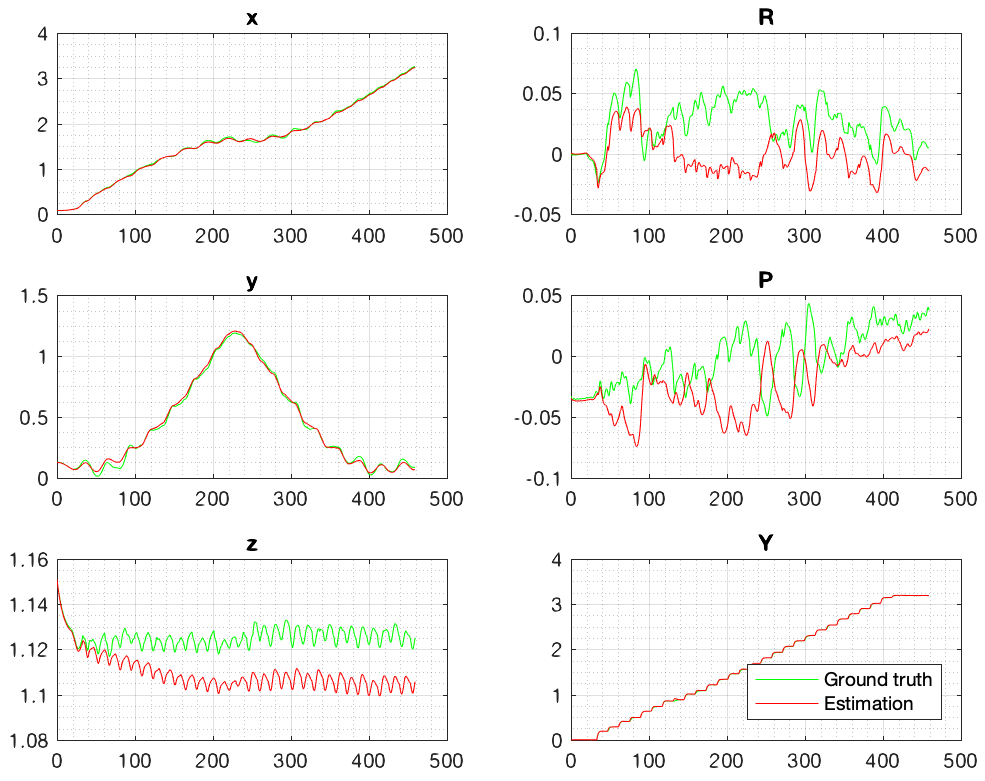
\includegraphics[width=0.5\textwidth]{images/trilateration.png}
        \end{figure}
    \end{frame}

    \section{MPC Loop Closure}

    \begin{frame}{MPC Loop CLosure}
    	The MPC need the position of the CoM with respect to the support
        foot to close the loop.

    	We want to estimate the same position but with the support foot
        reference frame with roll e pitch (wrt world frame) equal to zero.
    \end{frame}

    \begin{frame}{MPC Loop CLosure}
    	\begin{figure}
    	    \centering
    	    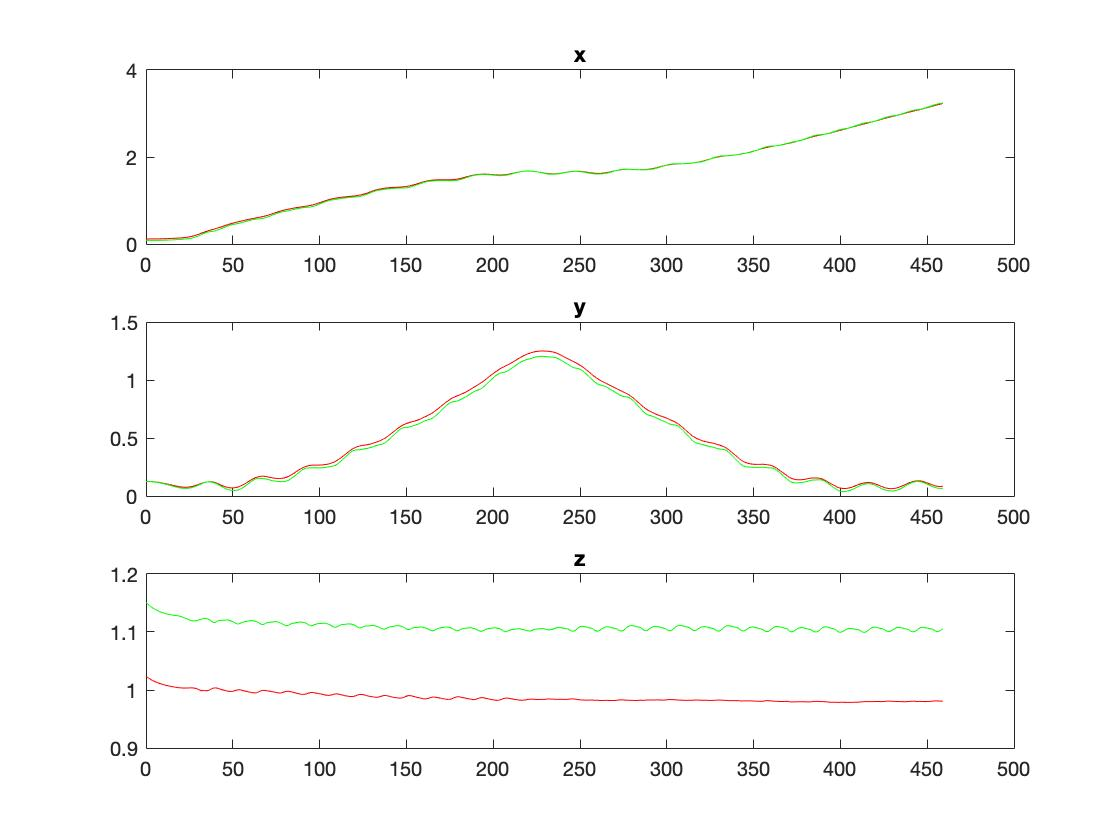
\includegraphics[scale=0.2]{images/comp_estimated_torso_com.jpg}
    	    \label{fig:my_label}
    	\end{figure}
    \end{frame}

    \begin{frame}{MPC Loop CLosure}
    	Given the estimate of the pose of the torso
        $(\bm{\hat{p}}_t, \bm{\hat{o}}_t)^T$,
        it is possible to obtain the estimate of the position of the support foot
        $(\bm{\hat{p}}_s, \bm{\hat{o}}_s)^T$  and of the CoM $(\bm{\hat{p}}_{CoM}, \bm{\hat{o}}_{CoM})^T$  using the kinematics relations.

        The position of the CoM in a rotated
        reference frame of the support foot $\mathcal{F}_{s'}$ which has the $z$-axis
        orthogonal to the floor is:

        \begin{equation*}
            \tensor[^{s'}]{\bm{\hat{p}}}{_{CoM}} = \bm{R}^{T}_{z}(\gamma)(\bm{\hat{p}}_{CoM}-\bm{\hat{p}}_{s})
        \end{equation*}

        This position can be used as a reference signal
        in the MPC in order to generate the gait of the humanoid robot.
    \end{frame}

    \section{Regulation}

    \begin{frame}{Kinematic Model of the Unicycle}
        Brief description:
        \begin{align*}
            \dot{x} &= v \text{cos}(\theta) \\
            \dot{y} &= v \text{sin}(\theta) \\
            \dot{\theta} &= \omega
        \end{align*}
        with $v$ and $\omega$ respectively linear and angular velocity.
    \end{frame}

    \begin{frame}{Proportional Controller}
        \justifying
        Control law:
        \begin{align*}
            v &= k_1 \left\| \bm{p}_g - \bm{\hat{p}}_t \right\| \\
            \omega &= k_2 e_{\theta}
        \end{align*}
        with $e_\theta$ angle between the sagittal vector of the unicycle
        and the vector pointing from the unicycle towards the goal, $k_1 =
        0.18$ and $k_2 = 0.014$. Forcing $v$ and $\omega$ to zero when
        $\left\|\bm{p}_g - \bm{\hat{p}}_t \right\| < 0.25$.
        Desired and final configuration:
        \begin{align*}
            \bm{q}_g &= (-3, 5, \cdot)^T \\
            \bm{q}_f &= (-2.798, 5.090, 0.98\pi)^T \\
            \bm{\hat{q}}_f &= (-2.885, 5.127, 0.979\pi)^T
        \end{align*}
    \end{frame}

    %\begin{frame}{Proportional Controller}
    %    Desired and final configuration:
    %    \begin{align*}
    %        \bm{q}_g &= (-3, 5, \cdot)^T \\
    %        \bm{q}_f &= (-2.798, 5.090, 0.98\pi)^T \\
    %        \bm{\hat{q}}_f &= (-2.885, 5.127, 0.979\pi)^T
    %    \end{align*}
    %\end{frame}

    \begin{frame}{Proportional Controller: x-y Plot}
        \begin{figure}
            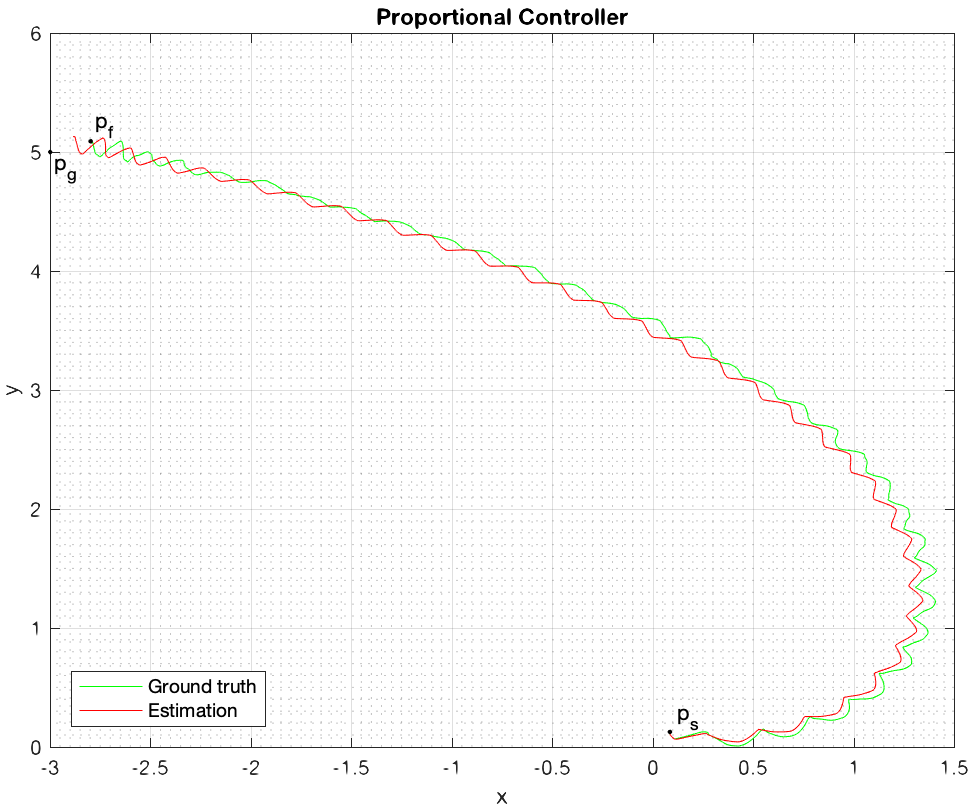
\includegraphics[width=0.85\textwidth]{images/proportional_controller.png}
        \end{figure}
    \end{frame}

    \begin{frame}{Cartesian Regulation}
        \justifying
        Let's express the coordinates of the unicycle in a reference frame
        $\mathcal{F}_g$ fixed at a position $(x_g, y_g)^T$ and
        rotated by $\theta_g$ around $\mathcal{F}_w$:
        \begin{equation*}
            \begin{pmatrix}
                \tensor[^g]{x}{} \\
                \tensor[^g]{y}{} \\
                \tensor[^g]{\theta}{}
            \end{pmatrix}
                =
            \bm{R}_z^T(\theta_g)
            \begin{pmatrix}
                x - x_g \\
                y - y_g \\
                \theta - \theta_g
            \end{pmatrix}
        \end{equation*}
    \end{frame}

    \begin{frame}{Cartesian Regulation}
        \justifying
        Control law:
        \begin{align*}
            v &= -k_1 (\tensor[^g]{x}{} \text{cos}(\tensor[^g]{\theta}{}) + \tensor[^g]{y}{} \text{sin}(\tensor[^g]{\theta}{})) \\
            \omega &=  k_2 (\text{Atan2}(\tensor[^g]{y}{}, \tensor[^g]{x}{}) - \tensor[^g]{\theta}{} + \pi)
        \end{align*}
        with $k_1 = 0.07$ and $k_2 = 0.01$. Forcing $v$ and $\omega$ to zero when
        $\left\|\bm{p}_g - \bm{\hat{p}}_t \right\| < 0.2$.
        Desired and final configuration:
        \begin{align*}
            \bm{q}_g &= (-2, 3.2, \cdot)^T \\
            \bm{q}_f &= (-1.788, 3.105, 1.562\pi)^T \\
            \bm{\hat{q}}_f &= (-1.823, 3.108, 1.562\pi)^T
        \end{align*}
    \end{frame}

    \begin{frame}{Cartesian Regulation: x-y Plot}
        \begin{figure}
            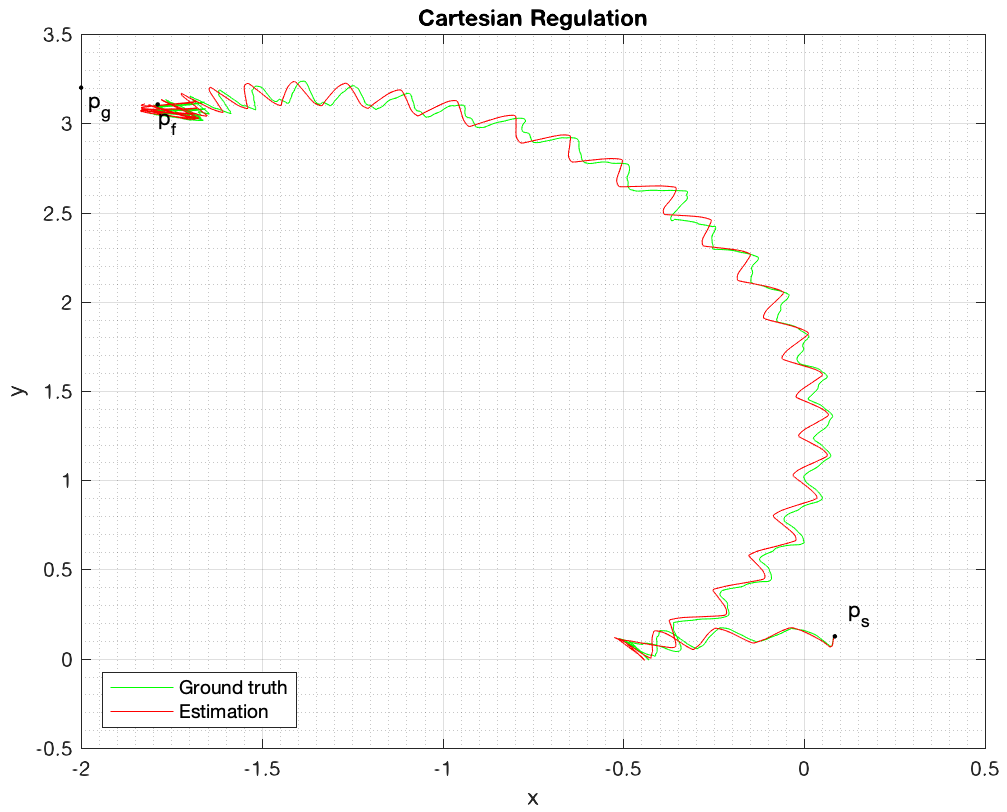
\includegraphics[width=0.85\textwidth]{images/cartesian_regulation.png}
        \end{figure}
    \end{frame}

    \begin{frame}{Kinematic Model of the Unicycle in Polar Coordinates}
        \justifying
        Brief description:
        \begin{align*}
            \dot{\rho}_r &= -v \text{cos}(\gamma_r) \\
            \dot{\gamma}_r &= \frac{\text{sin}(\gamma_r)}{\rho_r}v - \omega \\
            \dot{\delta}_r &= \frac{\text{sin}(\gamma_r)}{\rho_r}v
        \end{align*}
        Polar coordinates can be obtained from the generalized
        coordinates of the unicycle $(x, y, \theta)^T$ by computing:
        \begin{align*}
            \rho_r &= \sqrt{\tensor[^g]{x}{^2} + \tensor[^g]{y}{^2}} \\
            \gamma_r &= \text{Atan2}(\tensor[^g]{y}{}, \tensor[^g]{x}{}) - \tensor[^g]{\theta}{} + \pi \\
            \delta_r &= \gamma_r + \tensor[^g]{\theta}{}
        \end{align*}
    \end{frame}

    \begin{frame}{Posture Regulation}
        \justifying
        Control law:
        \begin{align*}
            v &= k_1 \rho_r \text{cos}(\gamma_r) \\
            w &= k_2 \gamma_r + k_1 \frac{\text{sin}(\gamma_r) \text{cos}(\gamma_r)}{\gamma_r}(\gamma_r + k_3 \delta_r)
        \end{align*}
        with $k_1 = 0.1$, $k_2 = 0.007$ $k_3 = 0.004$. Forcing $v$ and $\omega$ to zero when
        $\rho_r < 0.2$. Desired and final configuration:
        \begin{align*}
            \bm{q}_g &= (-2, 3.2, \pi)^T \\
            \bm{q}_f &= (-1.797, 3.194, 1.024\pi)^T \\
            \bm{\hat{q}}_f &= (-1.824, 3.222, 1.024\pi)^T \\
            \bm{\bar{q}}_f &= (-1.282, 3.424, 0.912\pi)^T
        \end{align*}
    \end{frame}

    \begin{frame}{Posture Regulation: x-y Plot}
        \begin{figure}
            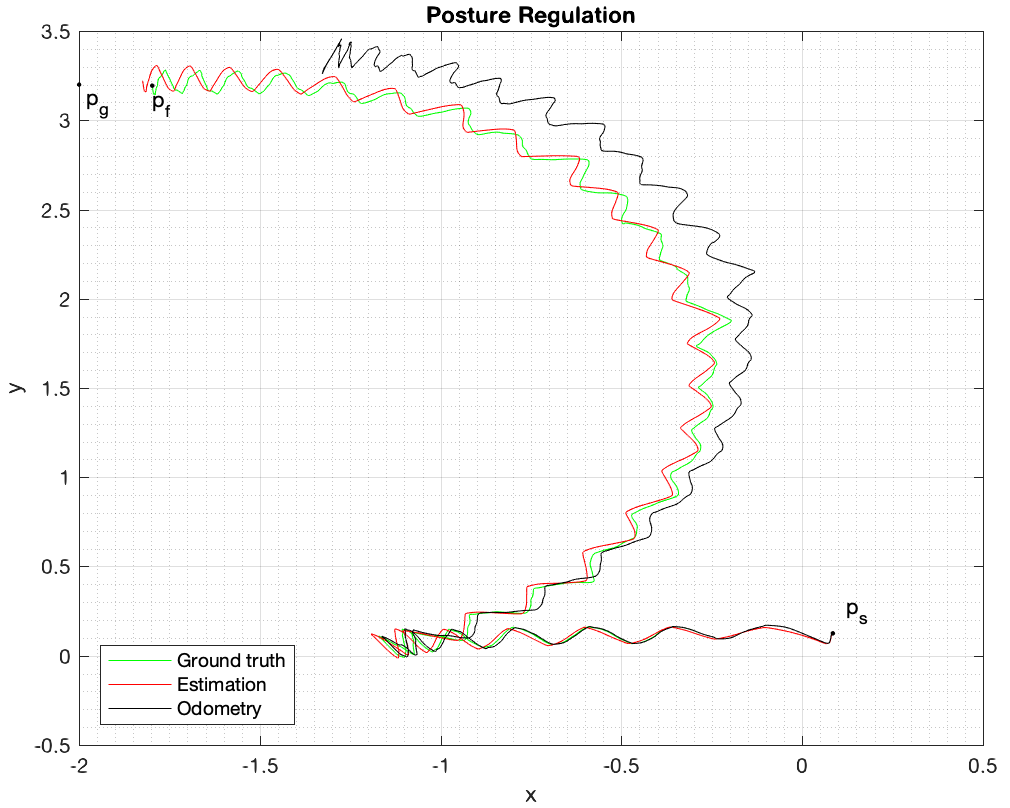
\includegraphics[width=0.85\textwidth]{images/posture_regulation.png}
        \end{figure}
    \end{frame}

    \begin{frame}{Posture Regulation: Yaw Plot}
        \begin{figure}
            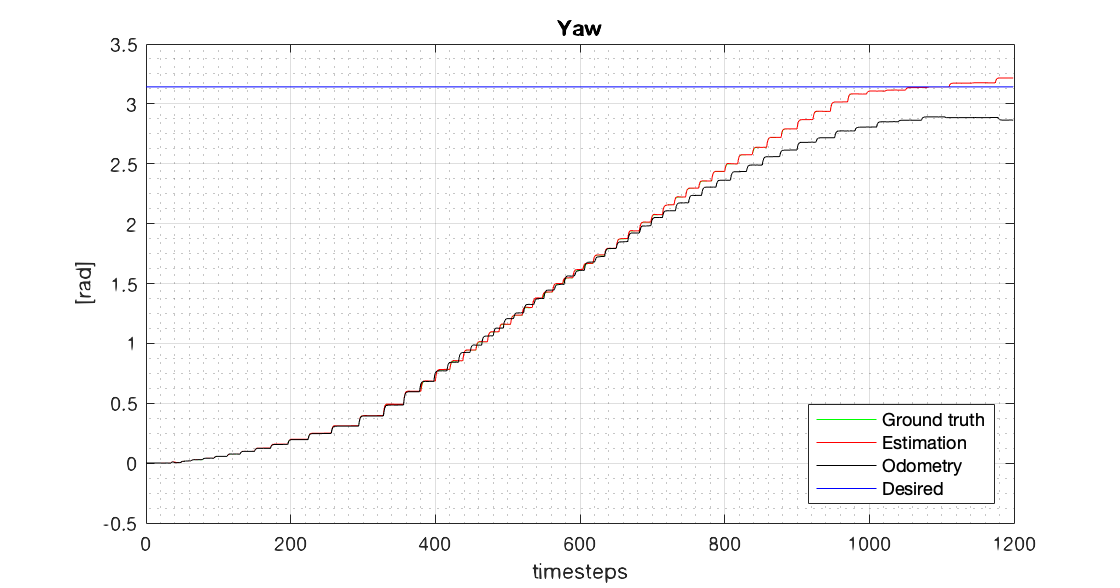
\includegraphics[width=\textwidth]{images/yaw_postureregulation.png}
        \end{figure}
    \end{frame}

    \begin{frame}{Posture Regulation: Velocity Profile Plots}
        \begin{figure}
            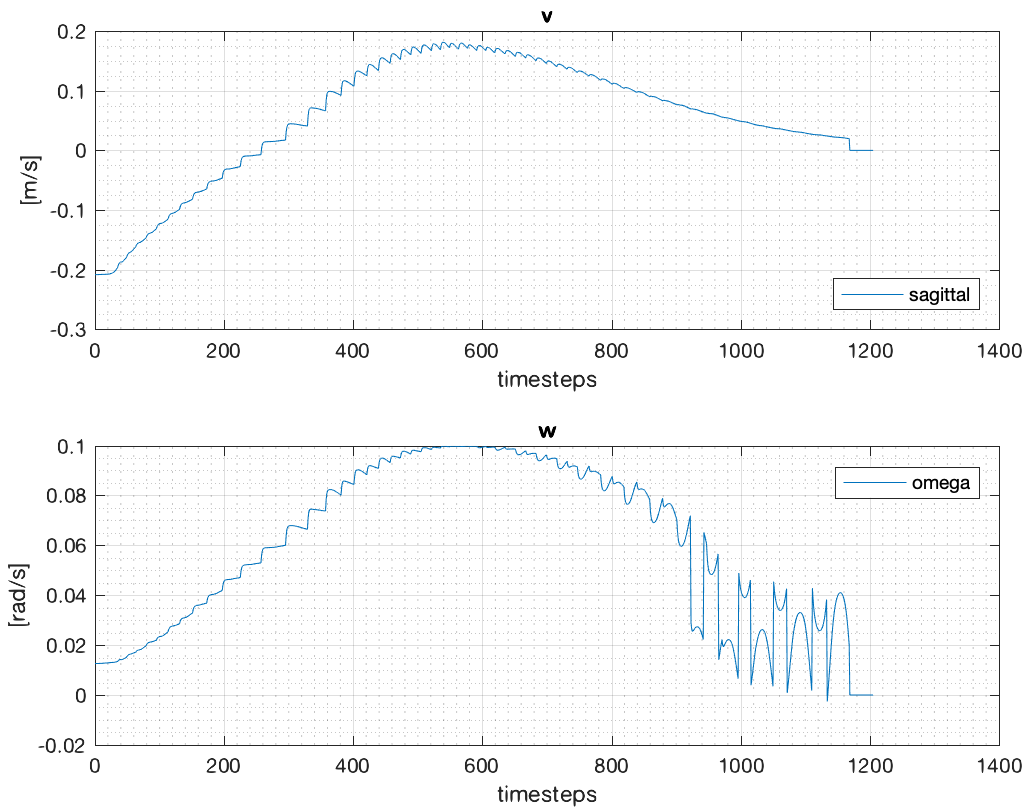
\includegraphics[width=0.9\textwidth]{images/unicycle_velocities.png}
        \end{figure}
    \end{frame}

    \begin{frame}{Conclusion}
        Conclusion.
    \end{frame}

    \begin{frame}[standout]
        Q\&A
    \end{frame}

    \appendix

    \begin{frame}{References}
        \bibliography{bibliography}
        \bibliographystyle{ieeetr}
    \end{frame}

\end{document}
